\section{Sensitivity Analysis}
Recall the fractional dynamic system that is being studied
\begin{equation}\label{eq:mainSystem}
	    \begin{array}{ll}
            \dfrac{d^{\alpha}X}{dt^{\alpha}}&=Z+(Y-a)X\\
            \dfrac{d^{\alpha}Y}{dt^{\alpha}}&=1-bY-X^2\\
            \dfrac{d^{\alpha}Z}{dt^{\alpha}}&=-X-cZ
        \end{array} \qquad \alpha\in(0,1]
\end{equation}
The main goal is measure the sensibility of parameters $a$, $b$ and $c$ as in \cite{guo2016sensitivity}.


For our first simulation, we will be analyzing the commensurate system (i.e same derivative order), $\alpha=0.84$ will be used. The initial values for the parameters are ($\mu_0$): $a_0=3$, $b_0=0.1$ and $c_0=1$. In order to calculate the behavior of $X$, $Y$ and $Z$ respect to $a$, $b$ and $c$, the associated Jacobian matrices are required. Let x be the vector of the state variables and $\mu$ the vector of parameters; hence,
\begin{equation}
	P(t,\mu_0)=\dfrac{\partial f}{\partial x}\Bigr|_{\mu_0} = \left[\begin{array}{ccc}
	Y-3 &\quad X 	&\quad 1\\ 
    -2X 	&\quad -0.1 	&\quad 0\\
    -1 		&\quad 0 	&\quad 1
	\end{array}\right] \qquad\qquad
    Q(t,\mu_0)=\dfrac{\partial f}{\partial \mu}\Bigr|_{\mu_0} = \left[\begin{array}{ccc}
	-X &\quad 0 	&\quad 0\\ 
    0  &\quad -Y 	&\quad 0\\
    0  &\quad 0 	&\quad -Z
	\end{array}\right]
\end{equation}

Let the sensitivity function

\begin{equation}
	S(t) = \dfrac{\partial f}{\partial x}\Bigr|_{\mu_0} = \left[
    \begin{array}{ccc}
		\dfrac{\partial X}{\partial a} &\quad \dfrac{\partial X}{\partial b} &\quad \dfrac{\partial X}{\partial c}\\
        \dfrac{\partial Y}{\partial a} &\quad \dfrac{\partial Y}{\partial b} &\quad \dfrac{\partial Y}{\partial c}\\
        \dfrac{\partial Z}{\partial a} &\quad \dfrac{\partial Z}{\partial b} &\quad \dfrac{\partial Z}{\partial c}
    \end{array}
    \right]\triangleq\left[
    \begin{array}{ccc}
		X_a&\quad  X_b&\quad X_c\\
        Y_a&\quad  Y_b&\quad Y_c\\
        Z_a&\quad  Z_b&\quad Z_c
    \end{array}
    \right]
\end{equation}

Where $S(t)$ contains the new state variables for our system. These variables measure how the state variables change respect to the parameters. Now, the sensitivity equation is defined as

\begin{equation}\label{eq:sensitivity}
	\begin{split}
      \dfrac{d^{0.84}S(t)}{dt^{0.84}} &= P(t,\mu_0)S(t) + Q(t,\mu_0)\\
      &=\left[\begin{array}{ccc}
      Y-3 &\quad X 	&\quad 1\\ 
      -2X 	&\quad -0.1 	&\quad 0\\
      -1 		&\quad 0 	&\quad 1
      \end{array}\right]     \left[\begin{array}{ccc}
          X_a&\quad  X_b&\quad X_c\\
          Y_a&\quad  Y_b&\quad Y_c\\
          Z_a&\quad  Z_b&\quad Z_c
      \end{array}\right]+\left[\begin{array}{ccc}
      -X &\quad 0 	&\quad 0\\ 
      0  &\quad -Y 	&\quad 0\\
      0  &\quad 0 	&\quad -Z
      \end{array}\right]
	\end{split}
\end{equation}

Now, combining the original system and the sensitivity equation, we obtain the new fractional dynamic system
\begin{equation}
	\begin{cases}
	\dfrac{d^{\alpha}X}{dt^{\alpha}}=Z+(Y-3)X, & X(0)=X_0\vspace{1.25mm}\\
    \dfrac{d^{\alpha}Y}{dt^{\alpha}}=1-0.1Y-X^2 & Y(0)=Y_0\vspace{1.25mm}\\
    \dfrac{d^{\alpha}Z}{dt^{\alpha}}=-X-Z & Z(0)=Z_0\vspace{1.25mm}\\
    \dfrac{d^{\alpha}X_a}{dt^{\alpha}}=Z_a-(1+Y_a)X-(3-Y)X_a & X_a(0)=0\vspace{1.25mm}\\
    \dfrac{d^{\alpha}X_b}{dt^{\alpha}}=Z_b+XY_b-(3-Y)X_b & X_b(0)=0\vspace{1.25mm}\\
    \dfrac{d^{\alpha}X_c}{dt^{\alpha}}=Z_c+XY_c-(3-Y)X_c & X_c(0)=0\vspace{1.25mm}\\
    \dfrac{d^{\alpha}Y_a}{dt^{\alpha}}=-0.1Y_a-2XX_a & Y_a(0)=0\vspace{1.25mm}\\
    \dfrac{d^{\alpha}Y_b}{dt^{\alpha}}=-Y-0.1Y_b-2XX_b & Y_b(0)=0\vspace{1.25mm}\\
    \dfrac{d^{\alpha}Y_b}{dt^{\alpha}}=-0.1Y_c-2XX_c & Y_b(0)=0\vspace{1.25mm}\\
    \dfrac{d^{\alpha}Z_a}{dt^{\alpha}}= -X_a -Z_a& Z_a(0)=0\vspace{1.25mm}\\
    \dfrac{d^{\alpha}Z_b}{dt^{\alpha}}= -X_b -Z_b& Z_b(0)=0\vspace{1.25mm}\\
    \dfrac{d^{\alpha}Z_c}{dt^{\alpha}}= -Z-X_c -Z_c& Z_c(0)=0
	\end{cases}
\end{equation}

Adams-Bashforth-Moulton predictor-corrector with $T=1000$, $N=10000$ and $(X_0,Y_0,Z_0)=(2,3,2)$ was used.

\begin{figure}[H]
        \centering
        \begin{subfigure}[b]{0.475\textwidth}
            \centering
            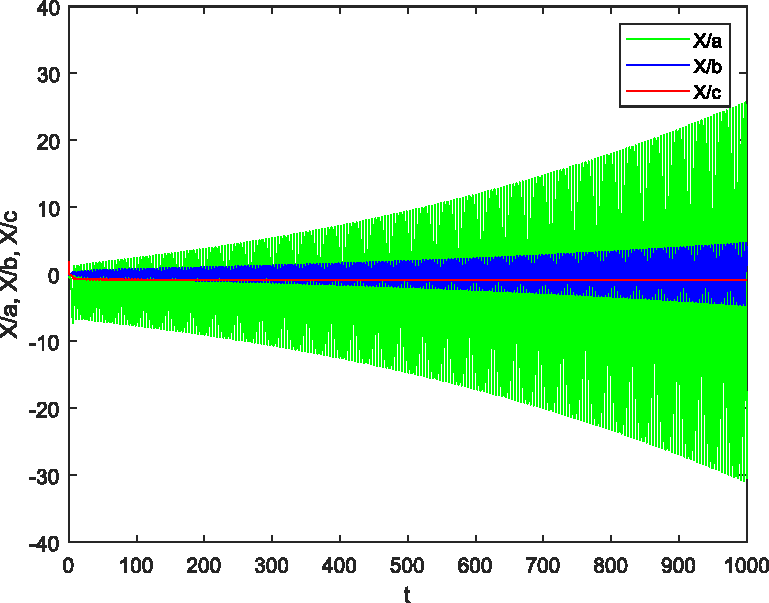
\includegraphics[scale=0.45]{files/dX_084.pdf}
            \caption{Change of X.}    
            \label{fig:dX_084}
        \end{subfigure}
        \hfill
        \begin{subfigure}[b]{0.475\textwidth}  
            \centering 
            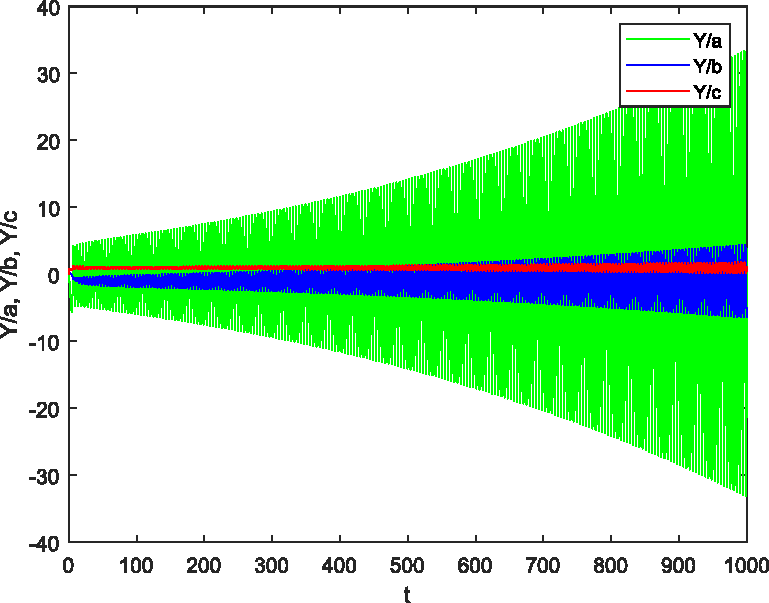
\includegraphics[scale=0.45]{files/dY_084.pdf}
            \caption{Change of Y.}  
            \label{fig:dY_084}
        \end{subfigure}
        \vskip\baselineskip
        \begin{subfigure}[b]{0.475\textwidth}   
            \centering 
            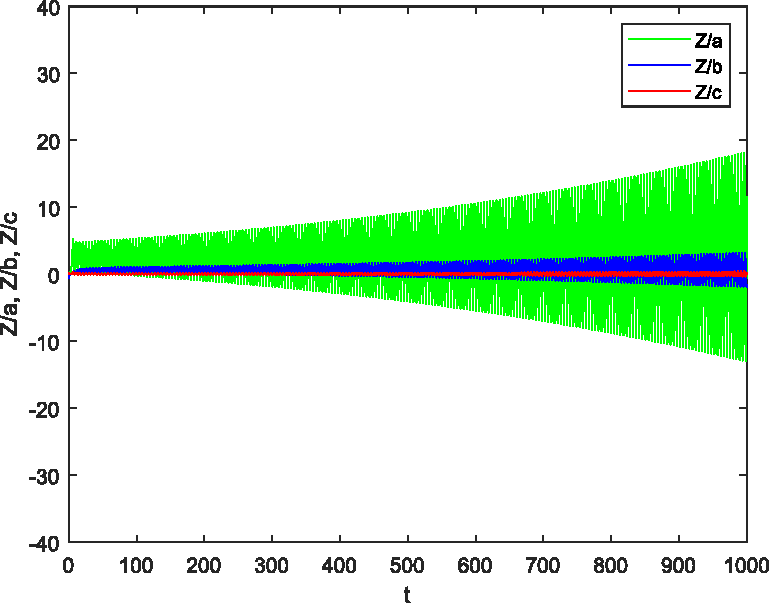
\includegraphics[scale=0.45]{files/dZ_084.pdf}
            \caption{Change of Z.}
            \label{fig:dZ_084}
        \end{subfigure}
        \caption{Changes of state variables respect to parameters.}
        \label{fig:d_084}
	\end{figure}
In figure \ref{fig:d_084}, the results for the sensitivity can be observed for $\alpha=0.84$. Note that, for all state variables, its change respect to $a$ is predominant over $b$ and $c$.

	\begin{figure}[H]
        \centering
        \begin{subfigure}[b]{0.475\textwidth}
            \centering
            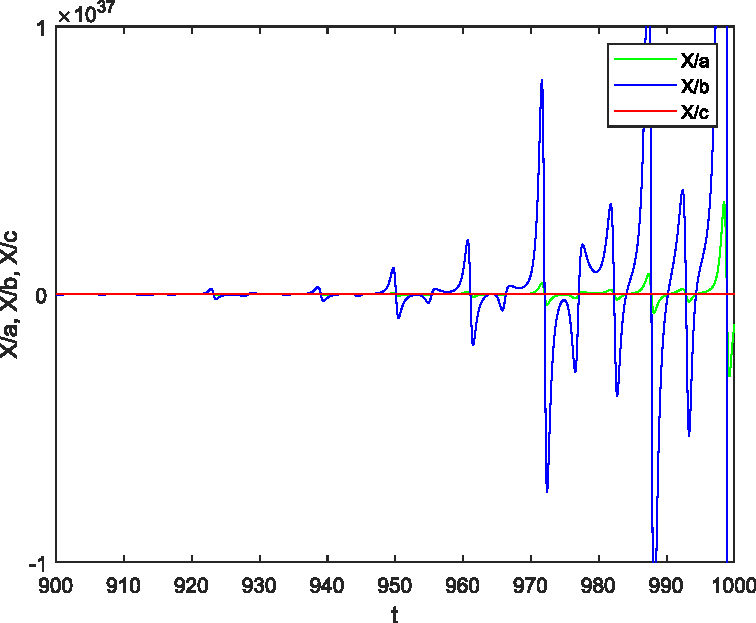
\includegraphics[scale=0.45]{files/dX_085.pdf}
            \caption{Change of X.}    
            \label{fig:dX_085}
        \end{subfigure}
        \hfill
        \begin{subfigure}[b]{0.475\textwidth}  
            \centering 
            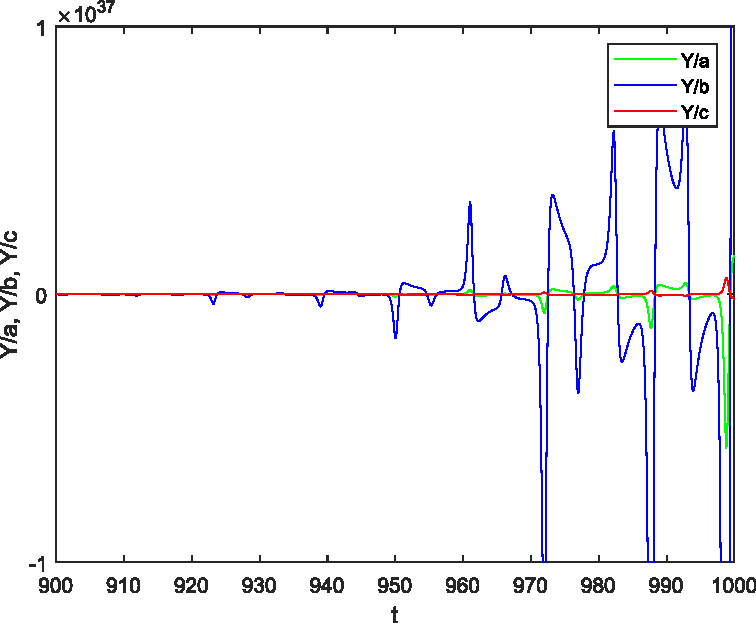
\includegraphics[scale=0.45]{files/dY_085.pdf}
            \caption{Change of Y.}  
            \label{fig:dY_085}
        \end{subfigure}
        \vskip\baselineskip
        \begin{subfigure}[b]{0.475\textwidth}   
            \centering 
            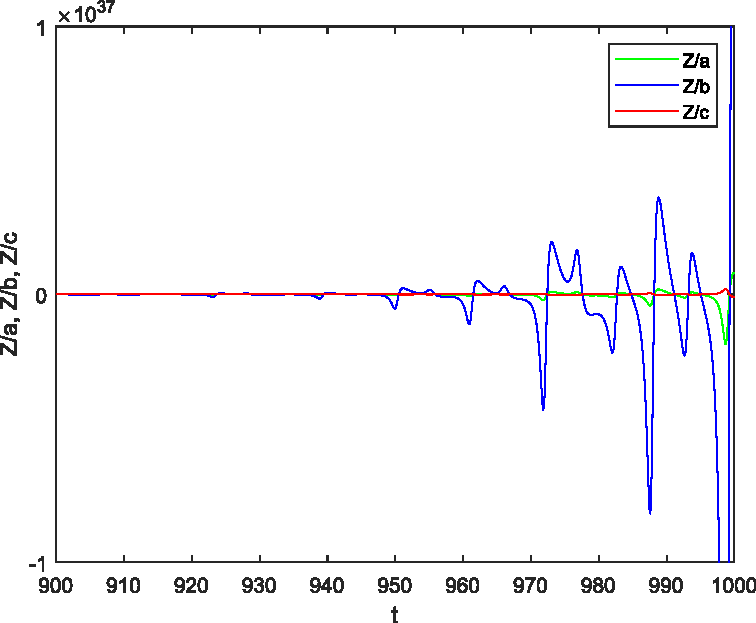
\includegraphics[scale=0.45]{files/dZ_085.pdf}
            \caption{Change of Z.}
            \label{fig:dZ_085}
        \end{subfigure}
        \caption{Changes of state variables respect to parameters.}
        \label{fig:d_085}
	\end{figure}
In figure \ref{fig:d_085}, the results for the sensitivity can be observed for $\alpha=0.85$. Note that, for all state variables, its change respect to $b$ is predominant over $a$ and $c$. Remark: the previous simulation was made with the same $T=1000$ and $N=10000$ as in the one with $\alpha=0.84$, but the plot was made only between $900\leq t\leq1000$ for a better visualization of system's behavior. 

Comparing the results for $\alpha=0.84$ and $\alpha=0.85$, it can be concluded that, in the first simulation, the system is not as sensitive as the one in the second simulation, since the rate of change for $b$ is in the order of $10^{
37}$ and for $a$ in the first one is in the order of $10^1$.

In figure \ref{fig:2a}, it can be seen the phase diagram for $\alpha=0.84$ and in section \ref{stab} it was proved that this system converges to a stable equilibrium point and the sensitivity analysis showed a bounded non-decreasing periodic behavior. 

In figure \ref{fig:2b}, it can be observed the phase diagram for $\alpha=0.85$ and in section \ref{stab} it was proved that this system has unstable equilibrium points and the sensitivity analysis showed a random oscillation, like a noise signal.

This suggests that there could be a relation between the stability of the system and its sensitivity.





